\documentclass[aspectratio=169,11pt]{beamer}
\usepackage[utf8]{inputenc}
\usepackage[T1]{fontenc}
\usepackage{graphicx}
\usepackage{booktabs}
\usepackage{tabularx}
\usepackage{ragged2e}
\usepackage{xcolor}
\usepackage{lmodern}
\pdfstringdefDisableCommands{\def\\{, }}

\definecolor{navy}{RGB}{13,35,64}
\definecolor{teal}{RGB}{0,145,150}
\definecolor{mist}{RGB}{239,244,248}
\setbeamercolor{normal text}{fg=navy,bg=white}
\setbeamercolor{frametitle}{fg=white,bg=navy}
\setbeamercolor{structure}{fg=teal}
\setbeamercolor{block title}{fg=white,bg=navy}
\setbeamercolor{block body}{fg=navy,bg=mist}
\setbeamercolor{block title alerted}{fg=white,bg=teal}
\setbeamercolor{block body alerted}{fg=navy,bg=mist}
\setbeamertemplate{navigation symbols}{}
\setbeamertemplate{footline}{%
  \hbox{\begin{beamercolorbox}[wd=.82\paperwidth,ht=2.7ex,dp=1.1ex,leftskip=1em]{author in head/foot}%
  \color{navy}\small RBlockSim | Computación Paralela y Distribuida\end{beamercolorbox}%
  \begin{beamercolorbox}[wd=.18\paperwidth,ht=2.7ex,dp=1.1ex,rightskip=1em plus1fil]{date in head/foot}%
  \color{navy}\small\insertframenumber/\inserttotalframenumber\end{beamercolorbox}}}
\setbeamertemplate{itemize item}{\color{teal}\raise0.2ex\hbox{\small$\blacktriangleright$}}
\setbeamertemplate{itemize subitem}{\color{teal}\raise0.2ex\hbox{\tiny$\bullet$}}
\setlength{\leftmargini}{1.25em}
\graphicspath{{figures/}}

\title{RBlockSim: reproducción de resultados}
\subtitle{Comparación visual con el paper original}
\author{Alva Cornejo, Jose Javier \and Carpio Paiva, Cesar Gonzalo\\
Palomino Rivadeneyra, Misael \and Zapana Pariapaza, Gonzalo Rodrigo}
\institute{Universidad Nacional de San Agustín}
\date{9 de noviembre de 2026}

\newcommand{\paperlabel}{\textbf{Paper original}}
\newcommand{\replabel}{\textbf{Reproducción (\texttt{\_1})}}
\newcommand{\compareblock}[1]{\vspace{.25em}\begin{alertblock}{Comparación}\small #1\end{alertblock}}

\begin{document}

\begin{frame}[plain]
  \vspace{.35cm}
  {\color{teal}\large COMPUTACIÓN PARALELA Y DISTRIBUIDA\par}
  \vspace{.2cm}
  {\color{navy}\LARGE\bfseries RBlockSim\par}
  {\color{navy}\Large Reproducción de resultados y comparación visual\par}
  \vspace{.35cm}\color{teal}\rule{.16\textwidth}{2pt}\par\vspace{.3cm}
  {\normalsize Alva Cornejo, Jose Javier\\
  Carpio Paiva, Cesar Gonzalo\\
  Palomino Rivadeneyra, Misael\\
  Zapana Pariapaza, Gonzalo Rodrigo\par}
  \vspace{.35cm}
  {\small Docente: ALVARO HENRY MAMANI ALIAGA\par}
  {\small Universidad Nacional de San Agustín\par}
  \vfill
  {\footnotesize Figuras reproducidas desde \texttt{reproduced/plots/plots\_1}.\\
  Referencia: Pimpini y Pellegrini, SIGSIM-PADS 2025.}
\end{frame}

\begin{frame}{Qué evalúa cada experimento}
\small
\begin{columns}[T,onlytextwidth]
\column{.49\textwidth}
\begin{block}{Ataques y validación}
\begin{itemize}
  \item \textbf{Fig. 3 — Validación:} comprueba si cada nodo mina bloques en proporción a su poder de hash.
  \item \textbf{Fig. 4 — Bloques aceptados:} cambia el hash del atacante; en selfish mining también varía tolerancia y profundidad.
  \item \textbf{Fig. 5 — Éxito selfish:} mide con qué frecuencia el ataque logra imponer la cadena oculta.
\end{itemize}
\end{block}
\column{.49\textwidth}
\begin{block}{Rendimiento y memoria}
\begin{itemize}
  \item \textbf{Fig. 6 — Tiempo:} cambia hilos, tamaño de red e intervalo de bloque; compara con CBlockSim.
  \item \textbf{Fig. 7 — Pico RAM:} observa la memoria máxima por configuración.
  \item \textbf{Fig. 8 — RAM agregada:} sigue el uso de memoria durante el avance de la simulación.
\end{itemize}
\end{block}
\end{columns}
\vspace{.3em}
\begin{center}\small Los ataques llegan a 10\,000 nodos; el rendimiento y la memoria incluyen 50\,000.\end{center}
\end{frame}

\begin{frame}{Metodología y entorno}
\footnotesize
\setlength{\itemsep}{2pt}
\begin{columns}[T,onlytextwidth]
\column{.48\textwidth}
\begin{block}{Campaña experimental}
\begin{itemize}
  \item Modo \texttt{all}: ataques, rendimiento y Figura 8.
  \item Ataques: 100, 1\,000 y 10\,000 nodos; 8 hilos; BI de 600\,s; 24\,h.
  \item Rendimiento y memoria: 100 a 50\,000 nodos; BI de 13\,s y 600\,s.
  \item Una iteración por configuración (el paper promedia cinco).
\end{itemize}
\end{block}
\column{.50\textwidth}
\begin{block}{Equipo y límites}
\begin{itemize}
  \item Intel Core i7-10850H: 6 núcleos / 12 hilos, 31\,GiB de RAM.
  \item Paper: 2$\times$ Xeon E5-2696 v4, 44/88 hilos, 256\,GB.
  \item Solo 1, 4 y 8 hilos son válidos; 16 o más fallan con \texttt{Demanding N cores (12)}.
  \item Ataques solo hasta 10\,000; 50\,000 en rendimiento y memoria.
\end{itemize}
\end{block}
\end{columns}
\compareblock{El hardware y la falta de repeticiones limitan los tiempos absolutos; las tendencias y los órdenes de magnitud sí son comparables.}
\end{frame}

\begin{frame}{Figura 3 · ¿el simulador respeta el poder de hash?}
\small\textbf{Experimento:} fracción de bloques minados frente a fracción de hash asignada.
\vspace{.2em}
\begin{columns}[T,onlytextwidth]
\column{.35\textwidth}\centering
\paperlabel\par\smallskip
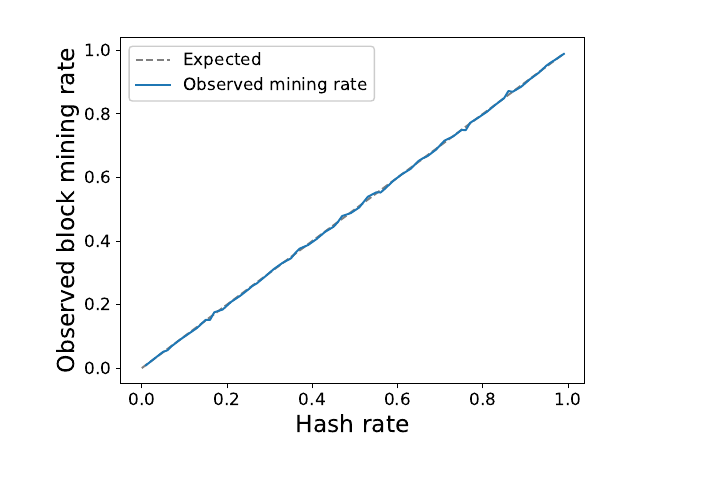
\includegraphics[width=\linewidth,height=2.8cm,keepaspectratio]{paper_original/figure3_hi.png}
\column{.63\textwidth}\centering
\replabel\par\smallskip
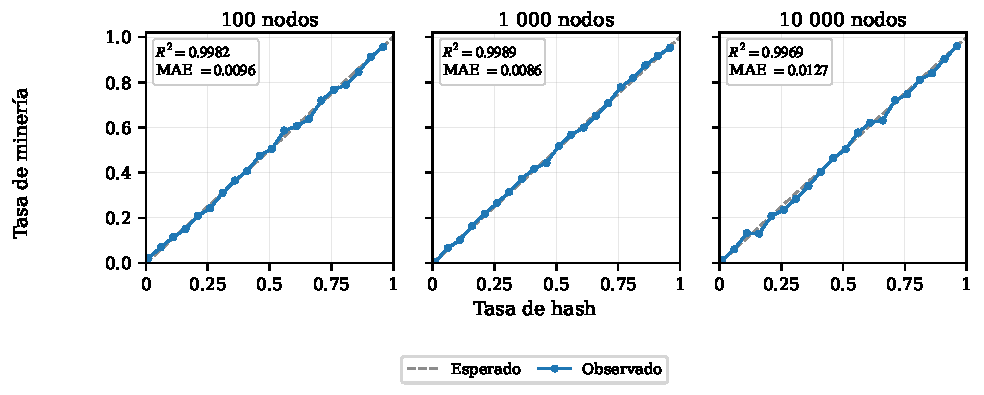
\includegraphics[width=\linewidth,height=2.8cm,keepaspectratio]{fig_validacion.pdf}
\end{columns}
\begin{block}{Métricas de la reproducción}
\centering\footnotesize
\begin{tabular}{lccc}
\toprule
Nodos & $R^2$ & MAE & RMSE \\
\midrule
100 & 0.9982 & 0.0096 & 0.0122 \\
1\,000 & 0.9989 & 0.0086 & 0.0095 \\
10\,000 & 0.9969 & 0.0127 & 0.0159 \\
\bottomrule
\end{tabular}
\end{block}
\end{frame}

\begin{frame}{Figura 4 (a--c) · ataque del 51\,\%}
\small\textbf{Experimento:} varía el hash del atacante y registra qué proporción de sus bloques termina en la cadena principal, para tres tamaños de red.
\vspace{.15em}
\begin{columns}[T,onlytextwidth]
\column{.49\textwidth}\centering
\paperlabel\par\smallskip
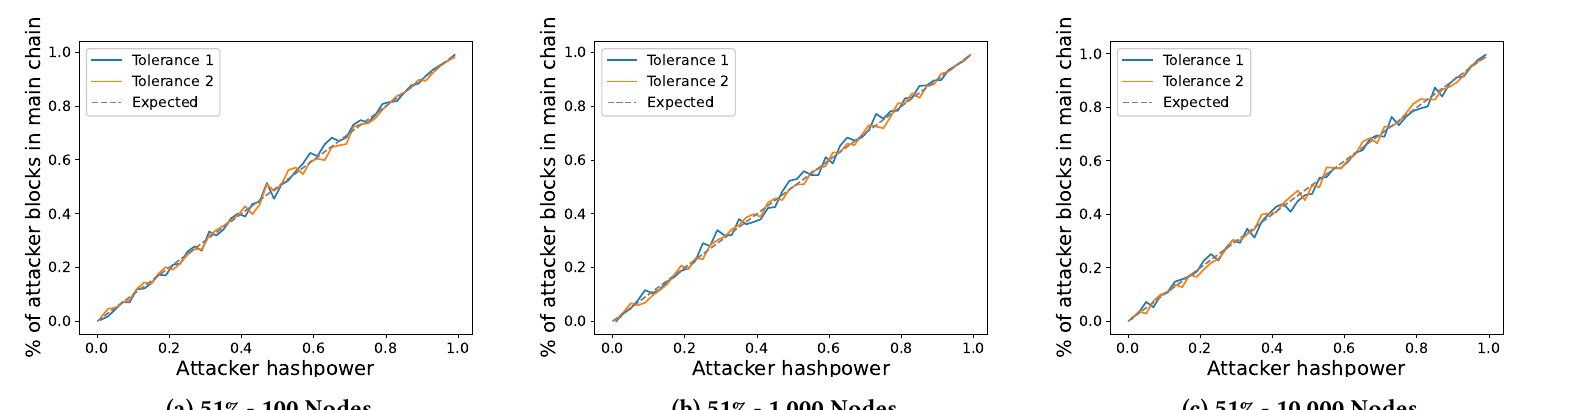
\includegraphics[width=\linewidth,height=3.5cm,keepaspectratio]{paper_original/figure4_51.png}
\column{.49\textwidth}\centering
\replabel\par\smallskip
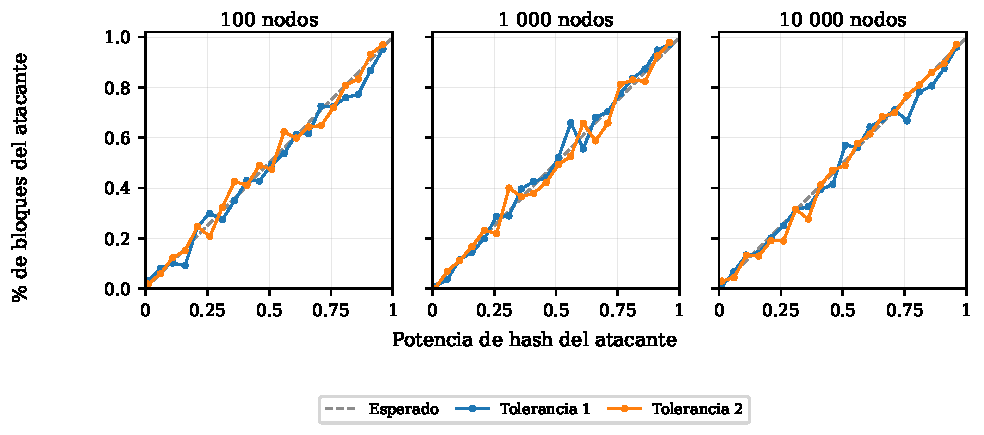
\includegraphics[width=\linewidth,height=3.5cm,keepaspectratio]{fig_51.pdf}
\end{columns}
\compareblock{Las dos tolerancias siguen la diagonal $y=x$ en 100, 1\,000 y 10\,000 nodos. MAE 0.020--0.031 y error máximo menor que 0.10: no se observa una aceptación desproporcionada del atacante.}
\end{frame}

\begin{frame}{Figura 4 (d--f) · bloques de selfish mining}
\small\textbf{Experimento:} varía hash, tolerancia al riesgo y profundidad del ataque; mide cuántos bloques del atacante se aceptan.
\vspace{.15em}
\begin{columns}[T,onlytextwidth]
\column{.49\textwidth}\centering
\paperlabel\par\smallskip
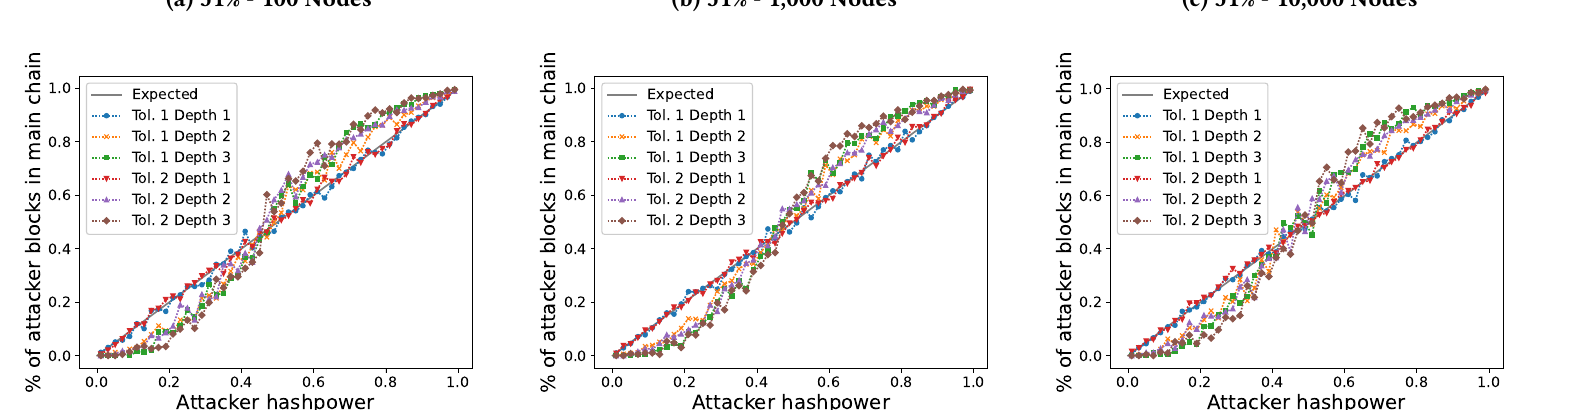
\includegraphics[width=\linewidth,height=3.5cm,keepaspectratio]{paper_original/figure4_selfish.png}
\column{.49\textwidth}\centering
\replabel\par\smallskip
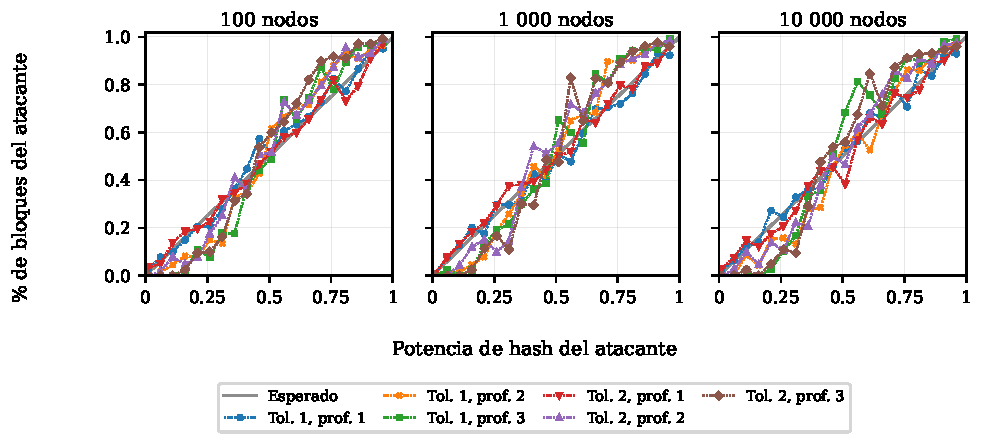
\includegraphics[width=\linewidth,height=3.5cm,keepaspectratio]{fig_selfish_committed.pdf}
\end{columns}
\compareblock{Se conserva el abanico de curvas y el efecto de la profundidad. El MAE crece de 0.024--0.032 (profundidad 1) a 0.063--0.081 (2) y 0.084--0.103 (3): a mayor profundidad, menos bloques comprometidos.}
\end{frame}

\begin{frame}{Figura 5 · probabilidad de éxito de selfish mining}
\small\textbf{Experimento:} cambia el hash del atacante y estima la frecuencia con que el ataque logra que los nodos honestos adopten la cadena oculta.
\vspace{.15em}
\begin{columns}[T,onlytextwidth]
\column{.49\textwidth}\centering
\paperlabel\par\smallskip
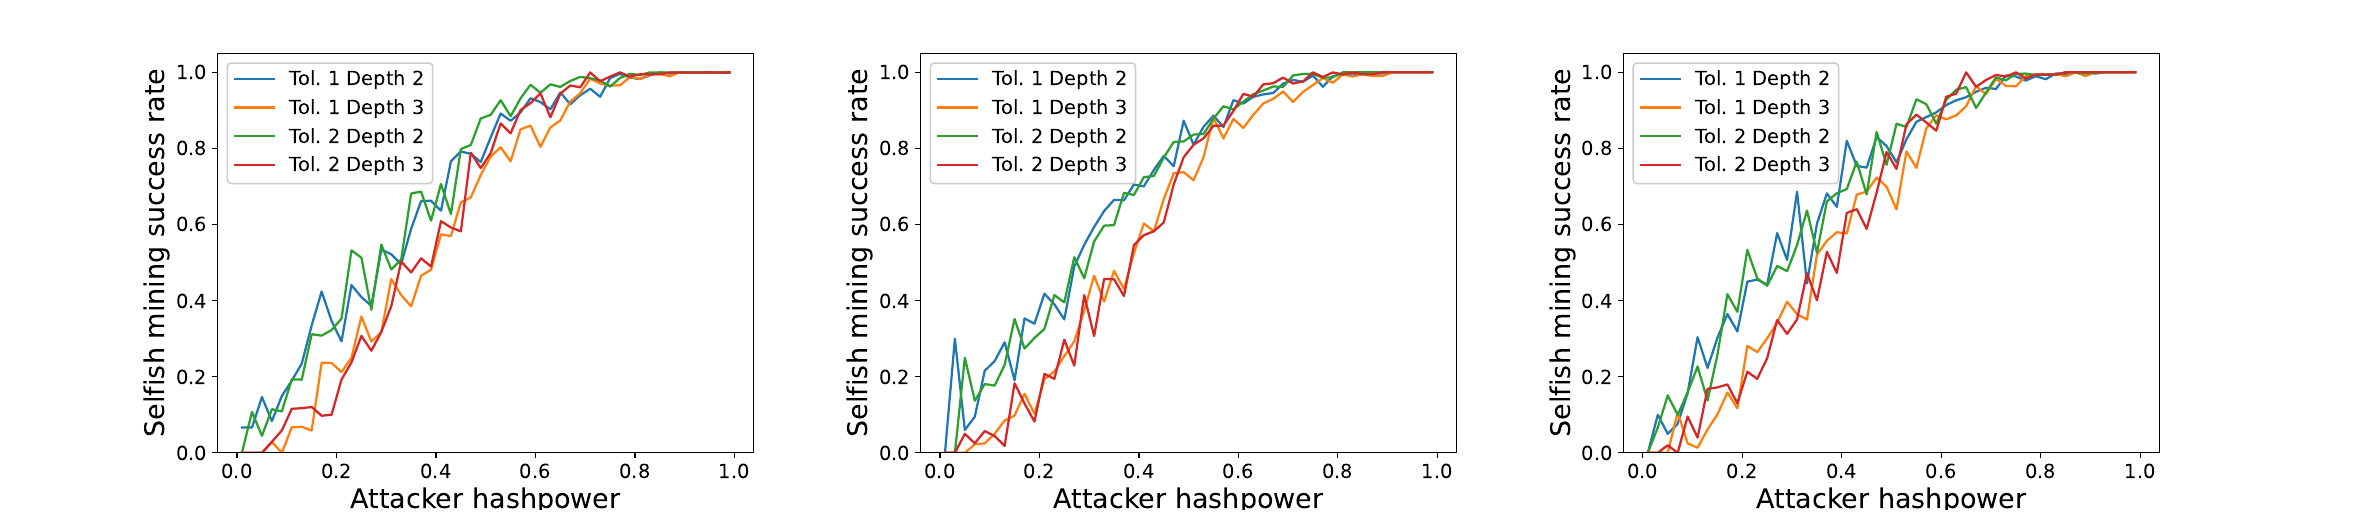
\includegraphics[width=\linewidth,height=3.2cm,keepaspectratio]{paper_original/figure5_hi.png}
\column{.49\textwidth}\centering
\replabel\par\smallskip
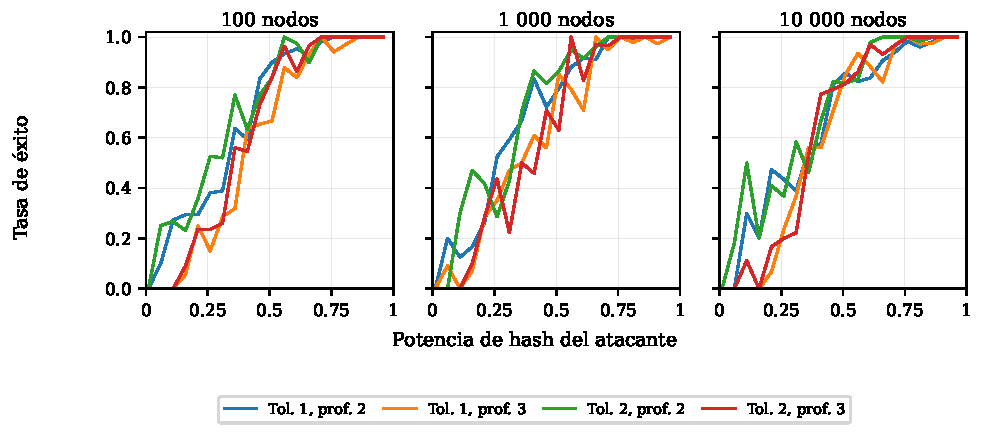
\includegraphics[width=\linewidth,height=3.2cm,keepaspectratio]{fig_selfish_success.pdf}
\end{columns}
\compareblock{La probabilidad sube con el hash y se satura para $h>0.75$ (0.94--1.00). En $h\approx0.51$ se obtiene 0.63--0.90; con hash bajo, 0.15--0.59. Las curvas reproducidas son más irregulares por usar una sola iteración.}
\end{frame}

\begin{frame}{Figura 6 · tiempo de ejecución}
\small\textbf{Experimento:} cambia hilos, tamaño de red e intervalo de bloque; registra el tiempo de reloj.
\vspace{.15em}
\begin{columns}[T,onlytextwidth]
\column{.49\textwidth}\centering
\paperlabel\par\smallskip
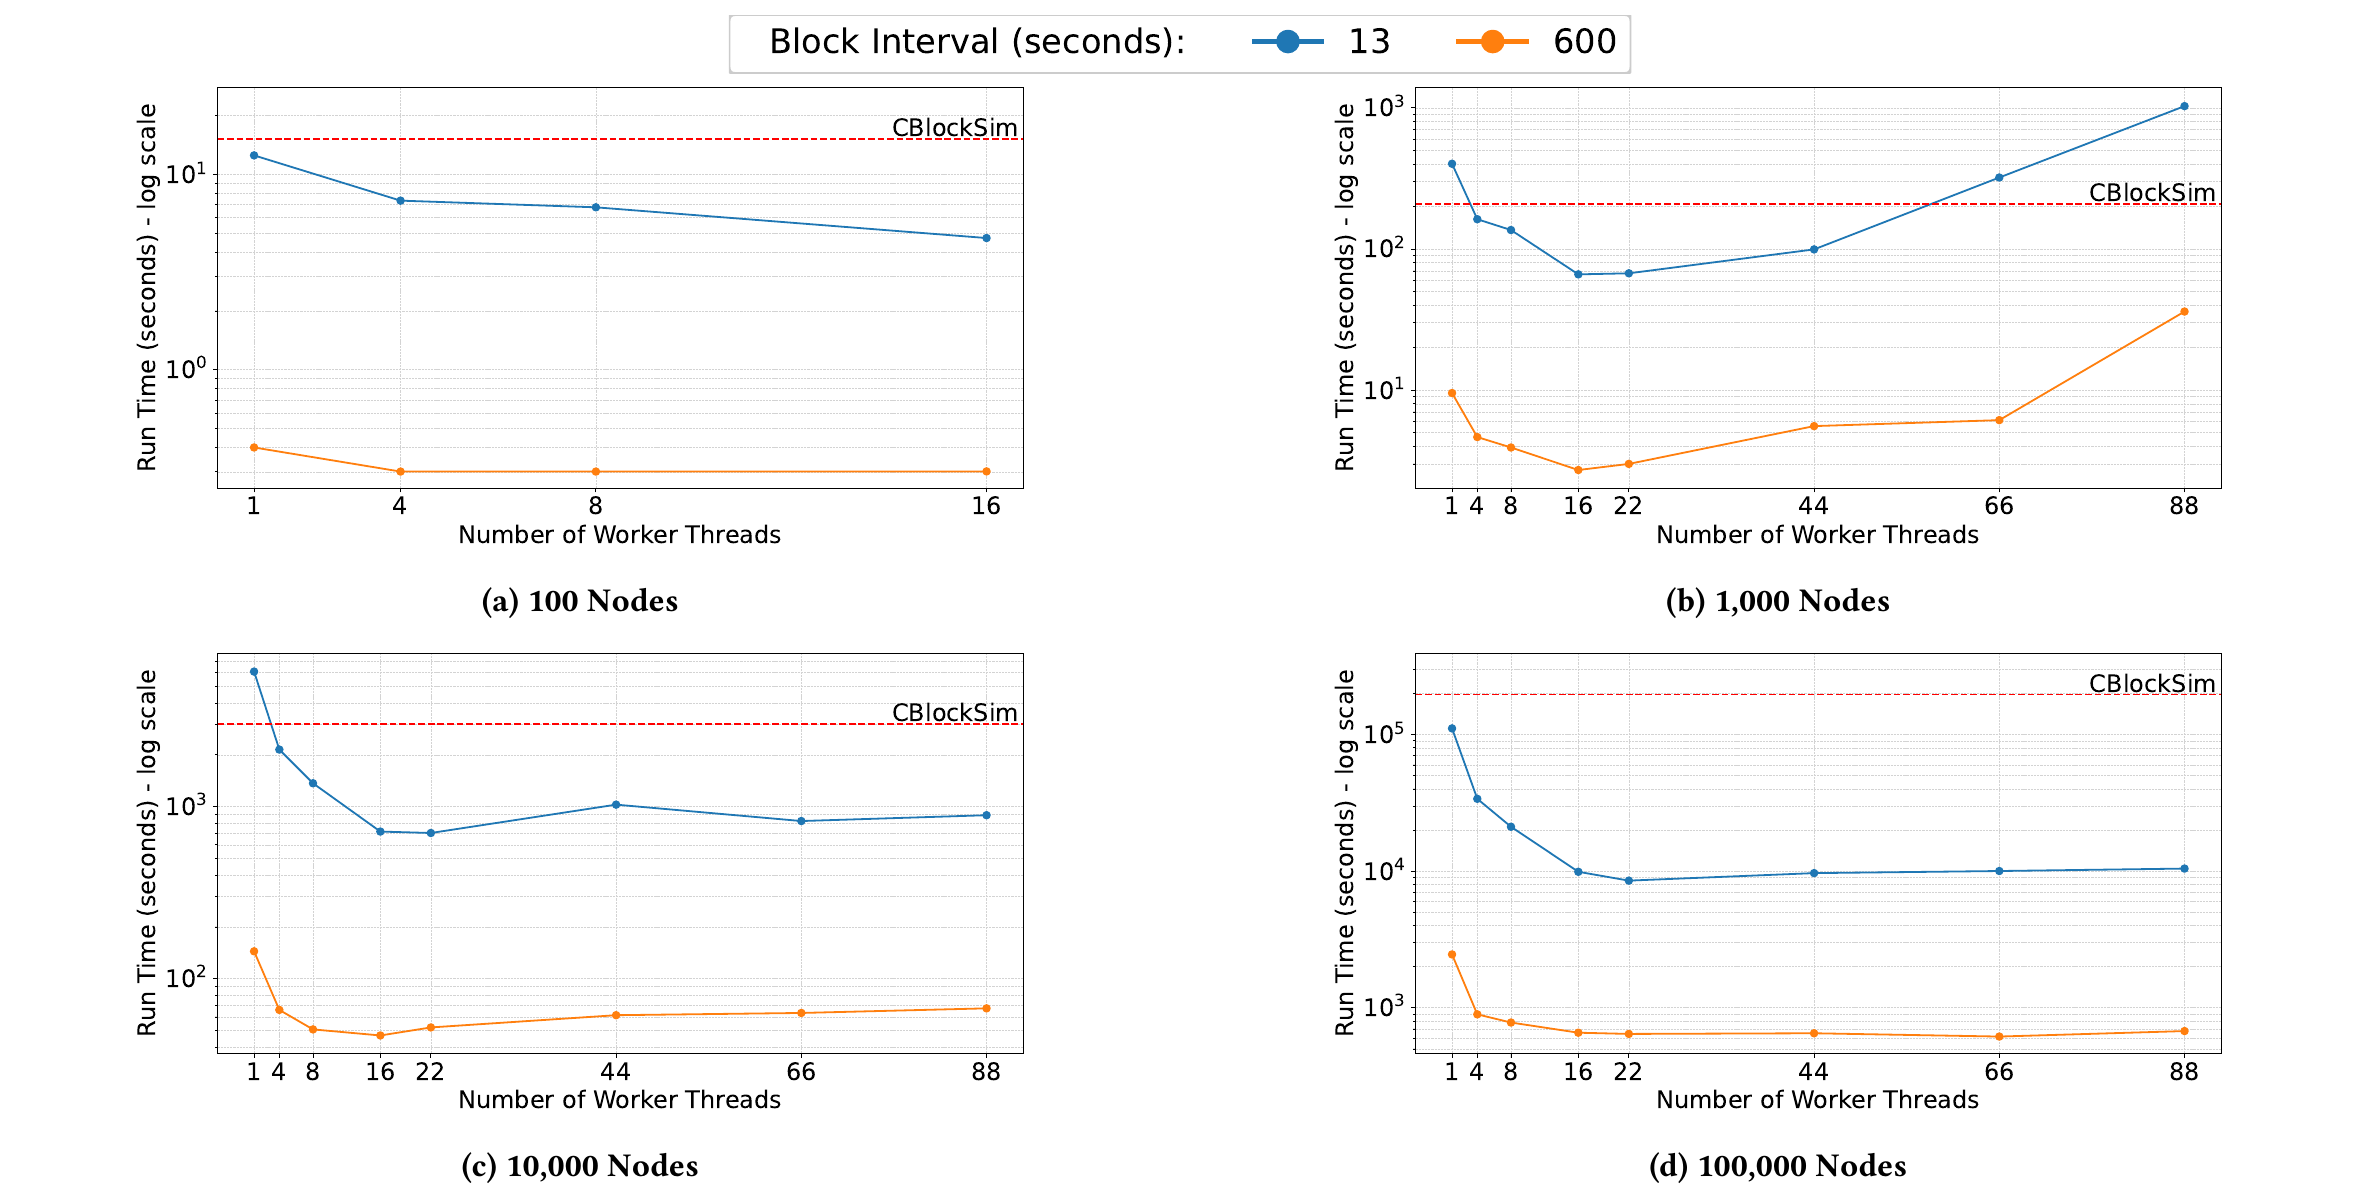
\includegraphics[width=\linewidth,height=3.9cm,keepaspectratio]{paper_original/figure6_hi.png}
\column{.49\textwidth}\centering
\replabel\par\smallskip
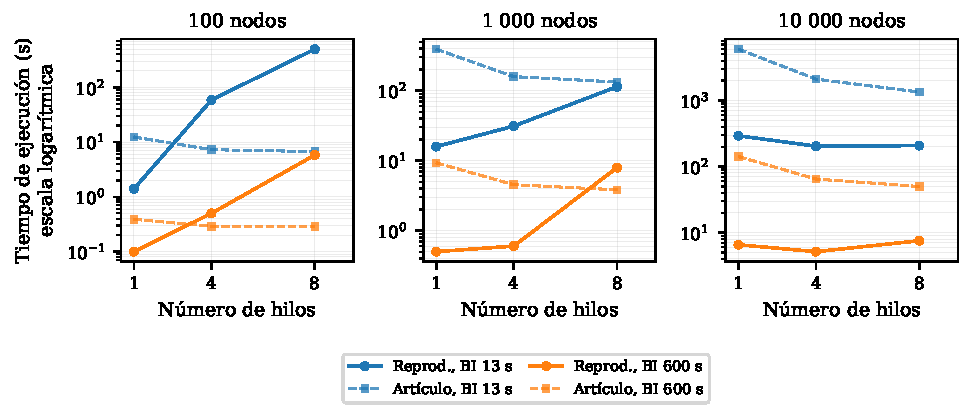
\includegraphics[width=\linewidth,height=3.9cm,keepaspectratio]{fig_performance_vs_paper.pdf}
\end{columns}
\compareblock{Solo 1, 4 y 8 hilos. En 100 y 1\,000 nodos el tiempo se degrada ($S(8)=0.003$ y 0.14); en 10\,000 y 50\,000 mejora hasta $1.44\times$ y $2.02\times$. No se puede verificar el pico de 16--22 hilos ni la referencia CBlockSim.}
\end{frame}

\begin{frame}{Figura 7 · pico de memoria}
\small\textbf{Experimento:} máximo de RAM al variar red, hilos e intervalo de bloque.
\vspace{.15em}
\begin{columns}[T,onlytextwidth]
\column{.44\textwidth}\centering
\paperlabel\par\smallskip
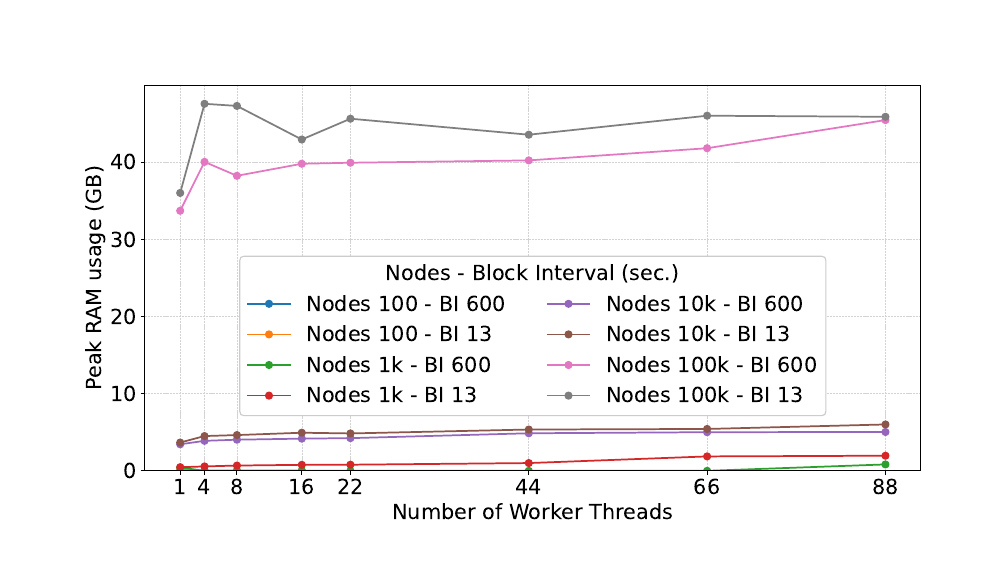
\includegraphics[width=\linewidth,height=3.6cm,keepaspectratio]{paper_original/figure7_hi.png}
\column{.54\textwidth}\centering
\replabel\par\smallskip
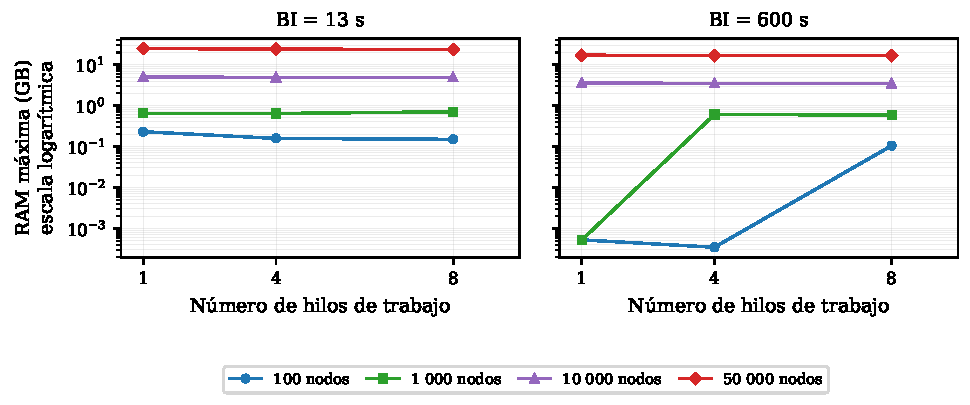
\includegraphics[width=\linewidth,height=3.6cm,keepaspectratio]{fig_ram.pdf}
\end{columns}
\compareblock{10\,000 nodos usan 3.5--5.0\,GB (paper: 3.4--5.9\,GB) y 50\,000, 16.6--24.9\,GB. El paper llega a 100\,000 nodos (35--47\,GB), escala no ejecutada.}
\end{frame}

\begin{frame}{Figura 8 · memoria a lo largo de la simulación}
\small\textbf{Experimento:} sigue el uso agregado de RAM conforme avanza la simulación.
\vspace{.15em}
\begin{columns}[T,onlytextwidth]
\column{.49\textwidth}\centering
\paperlabel\par\smallskip
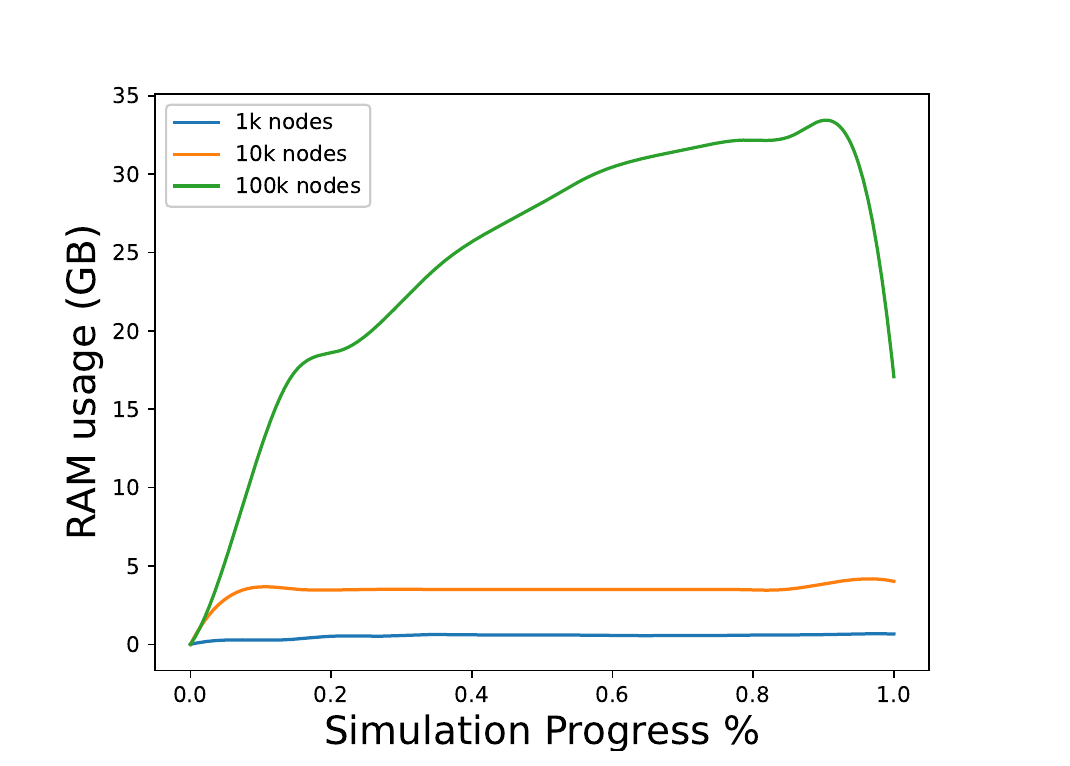
\includegraphics[width=\linewidth,height=3.7cm,keepaspectratio]{paper_original/figure8_hi.png}
\column{.49\textwidth}\centering
\replabel\par\smallskip
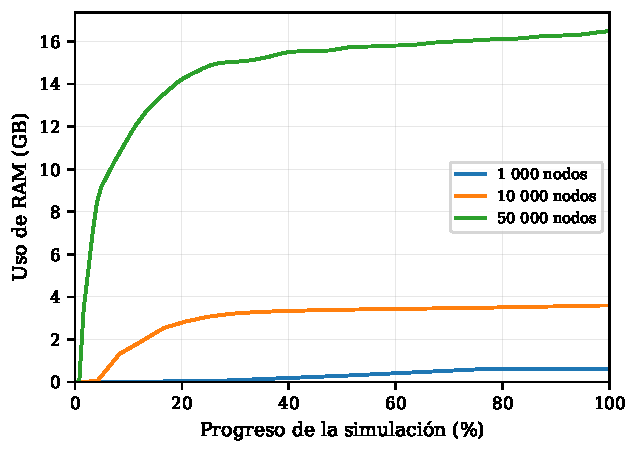
\includegraphics[width=\linewidth,height=3.7cm,keepaspectratio]{fig_ram_history.pdf}
\end{columns}
\compareblock{Mesetas: 0.6\,GB (1\,000 nodos), 3.6\,GB (10\,000) y 16.6\,GB (50\,000), con la misma forma de saturación. La caída final del original es el cierre de la simulación; la reproducción recorta ese tramo.}
\end{frame}

\begin{frame}{Estado de la reproducción por figura}
\scriptsize
\renewcommand{\arraystretch}{1.10}
\begin{tabularx}{\textwidth}{@{}l>{\raggedright\arraybackslash}X>{\raggedright\arraybackslash}X>{\raggedright\arraybackslash}p{2.5cm}@{}}
\toprule
\textbf{Figura} & \textbf{Artículo} & \textbf{Reproducción} & \textbf{Estado} \\
\midrule
3 & Tasa de minería proporcional al hash & $R^2 \ge 0.9969$, MAE $\le 0.0127$ & Conforme \\
4a--4c & 51\,\% sigue la diagonal & MAE 0.020--0.031 & Conforme \\
4d--4f & Selfish; la profundidad 3 compromete menos & Tendencias equivalentes & Conforme (cualitativo) \\
5 & Éxito crece con $h$ y se satura & Curvas equivalentes, más irregulares & Conforme (cualitativo) \\
6 & Pico de rendimiento en 16--22 hilos & Solo 1, 4 y 8 hilos; $S$ hasta $2.02\times$ & Parcial \\
7 & 10k: 3.4--5.9\,GB; 100k: 35--47\,GB & 10k: 3.5--5.0\,GB; 50k: 16.6--24.9\,GB & Conforme en magnitud \\
8 & 1k: $\sim$1\,GB; 10k: 8--9\,GB; 100k: $\sim$35\,GB & 1k: 0.6\,GB; 10k: 3.6\,GB; 50k: 16.6\,GB & Parcial \\
\bottomrule
\end{tabularx}
\vspace{.4em}
\begin{center}\small Alta en validación y ataques; parcial en memoria y rendimiento.\end{center}
\end{frame}

\begin{frame}{Conclusiones}
\begin{itemize}
  \item \textbf{Validación estadística:} se reproduce con alta fidelidad ($R^2 \ge 0.9969$, MAE $\le 0.0127$). El modelo de Proof of Work es consistente con la distribución esperada.
  \item \textbf{Ataques:} el 51\,\% no muestra ventaja indebida (MAE 0.020--0.031); selfish mining conserva tendencias y el efecto de la profundidad (MAE 0.024--0.103).
  \item \textbf{Rendimiento:} reproducción parcial. Con 1, 4 y 8 hilos, 10\,000 y 50\,000 nodos mejoran hasta $2.02\times$; 100 y 1\,000 se degradan. El pico de 16--22 hilos no es verificable con 12 vCPU.
  \item \textbf{Memoria:} consistente en orden de magnitud. 10\,000 nodos: 3.5--5.0\,GB; 50\,000: 16.6--24.9\,GB; mesetas de 0.6, 3.6 y 16.6\,GB.
  \item \textbf{Límites:} una iteración por configuración, hardware menor y ausencia de la red de 100\,000 nodos.
\end{itemize}
\vfill
\begin{center}\color{teal}\large RBlockSim es funcionalmente reproducible; el rendimiento es la parte más sensible al entorno.\end{center}
\end{frame}

\end{document}
